\documentclass{article}
\usepackage{xcolor}
\usepackage{graphicx}
\usepackage{float}
\usepackage{tikz}
\usepackage{parskip}
\usepackage{amsmath}
\usepackage{amsthm}
\usepackage{amssymb}
\usepackage{mathtools}
\usepackage{fancyhdr}
\usepackage[%paperheight = 59.4cm,
            %paperwidth = 42cm,
            %includehead,
            nomarginpar,
            textwidth=15cm,
            headheight=10mm]{geometry}


\begin{document}
 
\pagestyle{fancy}
%\fancyhead{}\fancyfoot{}

\fancyhf[OHC]{Christopher Munoz WRH4 Optimization}
\textbf{Problem 2.2:} \\
Theorem: Let $Z$ be an $n$ x $r$ null-space matrix for the matrix $A$. If $Y$ is any invertible $r$ x $r$ matrix,  $\hat{Z} = ZY$ is also a null-space matrix for A.

Proof: Given that Z is an $n$ x $r$ null-space matrix for matrix $A$, we know that $AZ = 0$, we also know that $Y$ is an invertible matrix. We need to show that $A\hat{Z} = 0$ or $AZY = 0$ for $\hat{Z} = ZY$ to be a null-space matrix for A. Consider the following:
\begin{align*}
    A \hat{Z} = A(ZY) \\
    A(ZY) = (AZ)Y \\
    A(ZY) = 0Y \\
    AZY = 0 \text{ or } A\hat{Z} = 0
\end{align*}
Thus proving $\hat{Z} = ZY$ is also a null-space matrix for A. \newline

\textbf{Problem 3.1:} We will compute a basis for the null space for the following matrices(Denoted with A) using variable reduction:

\textbf{\{i\}}
\begin{align*} A =
    \begin{bmatrix}
        1 & 1 & 1 & 1 \\
        1 & -1 & -1 & 1 \\
        0 & 1 & 0 & 1
    \end{bmatrix} \Rightarrow
    \begin{bmatrix}
        1 & 1 & 1 & 1 \\
        0 & -2 & -2 & 0 \\
        0 & 1 & 0 & 1
    \end{bmatrix} && R_1 - R_2 \xrightarrow{} R_2 \\
    \begin{bmatrix}
        1 & 1 & 1 & 1 \\
        0 & -2 & -2 & 0 \\
        0 & 0 & -1 & 1
    \end{bmatrix} && \frac{R_2}{2} + R_3 \xrightarrow{} R_3 
\end{align*}\begin{align*}
    x_1 + x_2 + x_3 + x_4 = 0 && -2x_2 - 2x_3 = 0 && -x_3 + x_4 = 0 && x_4 = x_4 \\
    x_4 = t && x_3 = t && x_2 = -t && x_1 = -t
\end{align*}
Thus null(A) $ = t\begin{bmatrix} -1 \\ -1 \\ 1 \\ 1\end{bmatrix}$ for $t \in \mathbb{R}$ \newline

\textbf{\{ii\}}
\begin{align*} A = 
    \begin{bmatrix}
        1 & 1 & 1 & 1
    \end{bmatrix}
\end{align*}
\begin{align*}
    x_1 + x_2 + x_3 + x_4 = 0 &&
    x_2 = x_2 && x_3 = x_3 && x_4 = x_4 \\
    x_2 = s && x_3 = t && x_4 = u && x_1 = -s -t - u
\end{align*}
Thus null(A) $ = s\begin{bmatrix} -1 \\ 1 \\ 0 \\ 0\end{bmatrix} + t\begin{bmatrix} -1 \\ 0 \\ 1 \\ 0\end{bmatrix} +u\begin{bmatrix} -1 \\ 0 \\ 0 \\ 1\end{bmatrix} $   for $s,t,u \in \mathbb{R}$ \newline
\textbf{\{iii\}}
\begin{align*} A = 
    \begin{bmatrix}
        1 & 1 & 1 & 1 \\
        1 & -1 & -1 & 1
    \end{bmatrix} \Rightarrow
    \begin{bmatrix}
        1 & 1 & 1 & 1 \\
        0 & 2 & 2 & 0
    \end{bmatrix} && R_1 - R_2 \xrightarrow{} R_2
\end{align*}
\begin{align*}
    x_1+x_2+x_3+x_4 = 0 && 2x_2 + 2x_3 = 0 && x_3 = s && x_4 = t \\
    x_2 = -x_3 = -s && x_1 - s + s + t = 0 && x_1 = s - s - t && x_1 = -t
\end{align*}
Thus null(A) $ = s\begin{bmatrix} 0 \\ -1 \\ 1 \\ 0\end{bmatrix} + t\begin{bmatrix} -1 \\ 0 \\ 0 \\ 1\end{bmatrix} $   for $s,t \in \mathbb{R}$ \newline

\textbf{\{iv\}}
\begin{align*} A =
    \begin{bmatrix}
        1 & 1 & 1 & 1 \\
        2 & 0 & 0 & 2 \\
        1 & -1 & -1 & 1
    \end{bmatrix} \Rightarrow
    \begin{bmatrix}
        1 & 1 & 1 & 1 \\
        2 & 0 & 0 & 2 \\
        0 & -1 & -1 & 0
    \end{bmatrix} && \frac{R_2}{2} - R_3 \xrightarrow{} R_3 \\
    \begin{bmatrix}
        1 & 1 & 1 & 1 \\
        0 & 2 & 2 & 0 \\
        0 & -1 & -1 & 0
    \end{bmatrix} && 2R_1 - R_2 \xrightarrow{} R_2 \\
    \begin{bmatrix}
        1 & 1 & 1 & 1 \\
        0 & 2 & 2 & 0 \\
        0 & 0 & 0 & 0
    \end{bmatrix} 
    && \frac{R_2}{2} + R_3 \xrightarrow{} R_3 \\
    \begin{bmatrix}
        1 & 1 & 1 & 1 \\
        0 & 1 & 1 & 0 \\
        0 & 0 & 0 & 0
    \end{bmatrix} 
    && \frac{R_2}{2} \xrightarrow{} R_2 \\
    \begin{bmatrix}
        1 & 0 & 0 & 1 \\
        0 & 1 & 1 & 0 \\
        0 & 0 & 0 & 0
    \end{bmatrix}
    && R_2 - R_1 \xrightarrow{} R_1
\end{align*}
\begin{align*}
    x_1 + x_4 = 0 && x_2 + x_3 = 0 && x_3 = s && x_4 = t \\
    x_2 = -s && x_1 = -t
\end{align*} Thus null(A) $ = s\begin{bmatrix} 0 \\ -1 \\ 1 \\ 0\end{bmatrix} + t\begin{bmatrix} -1 \\ 0 \\ 0 \\ 1\end{bmatrix} $   for $s,t \in \mathbb{R}$ \newline

\textbf{Problem 3.3} For the following problem we use $p_2$ and $p_3$ as our basic variables for $A$ and we attempt the same with $p_1$ and $p_4$
\begin{align*} A = 
    \begin{bmatrix}
      1 & 2 & 0 & 2 \\
      2 & 2 & 1 & 4
    \end{bmatrix}
\end{align*}
\begin{align*}
    p_1 + 2p_2 + 2p_4 = 0 && 2p_1 + p_2 + 2p_3 + 4p_4 = 0 &&
    p_1 = -2p_2 - 2p_4 \\ -4p_2 - 4p_4 + p_2 + 2p_3 + 4p_4 = 0 && -3p_2 + 2p_3 = 0 && p_2 = \frac{2}{3}p_3 \\
    p_1 = -\frac{4}{3}p_3 - 2p_4
\end{align*}
    Since $p_2 = \frac{2}{3} p_3$ We end up using $p_4$ as our free variable
    \begin{align*}\text{null}(A) = 
    p_3
    \begin{bmatrix}
        -\frac{4}{3} \\ \frac{2}{3} \\ 1 \\ 0
    \end{bmatrix} +
    p_4
    \begin{bmatrix}
        -2 \\ 0 \\ 0 \\ 1
    \end{bmatrix}
\end{align*}
 For the second part of the problem we consider $p_1$ and $p_4$ as our free variables, we similarly reduce and substitute to get our vectors:
\begin{align*}
    p_1 + 2p_2 + 2p_4 = 0 && 2p_1 + p_2 + 2p_3 + 4p_4 = 0 && p_2 = - \frac{1}{2}(p_1 + 2p_4) \\
    2p_1 - \frac{1}{2}p_1 - p_4 + 2p_3 + 4p_4 = 0 && \frac{3}{2}p_1 + 2p_3 + 3p_4 = 0 && 2p_3 = -\frac{3}{2} - 3p_4 \\
    p_3 = -\frac{3}{4}p_1 - \frac{3}{2}p_4  
\end{align*}
    We can construct our solution with our $p_2= -\frac{1}{2}(p_1 + 2p_4)$ and $p_3 = -\frac{3}{4}p_1 - \frac{3}{2}p_4$
    \begin{align*}\text{null}(A) = p_1
    \begin{bmatrix}
        1 \\ -\frac{1}{2} \\ -\frac{3}{4} \\ 0
    \end{bmatrix}
        +  p_4
    \begin{bmatrix}
        0 \\ -1 \\ -\frac{3}{2} \\ 1
    \end{bmatrix}
\end{align*}
So we can actually do it with $p_1$ and $p_4$ as basic variables. \newline

\textbf{Problem 3.4} Theorem: Let $A$ be an $m$ x $n$ matrix of full row rank. The matrix $AA^T$ is positive definite and so its inverse exists. \newline 

    Proof: We want to show that $x^TAA^Tx > 0$ (using the definition of positive definite) for some non-zero vector $x \in \mathbb{R}^m$, first we note that $AA^T$ is symmetric:
\begin{align*}
    (AA^T)^T = (A^T)^TA^T = AA^T
\end{align*}
Now we consider the the case of $x^TAA^Tx$ 
\begin{align*}
    x^TAA^Tx = (A^Tx)^T(A^Tx) = ||A^Tx||^2
\end{align*}
    This is because the product of a vector and its transpose is the squared norm which is always positive. In our case as long as $x$ is a non-zero vector, $x^TAA^Tx$ is positive definite and thus invertible.

\textbf{problem 1.1} We solve the following linear programs graphically: \newline
\textbf{\{i\}}
    \begin{align*}
        \text{minimize} &\null \quad z = 3x_1 + x_2 \\ 
        \text{subject to} &\null \quad x_1 - x_2 \leq 1 \\
        & 3x_1 + 2x_2 \leq 12 \\
        & 2x_1 + 3x_2 \leq 3 \\
        & -2x_1 + 3x_2 \geq 9 \\
        & x_1, x_2 \geq 0
    \end{align*}
    \begin{figure}[H]
        \centering
        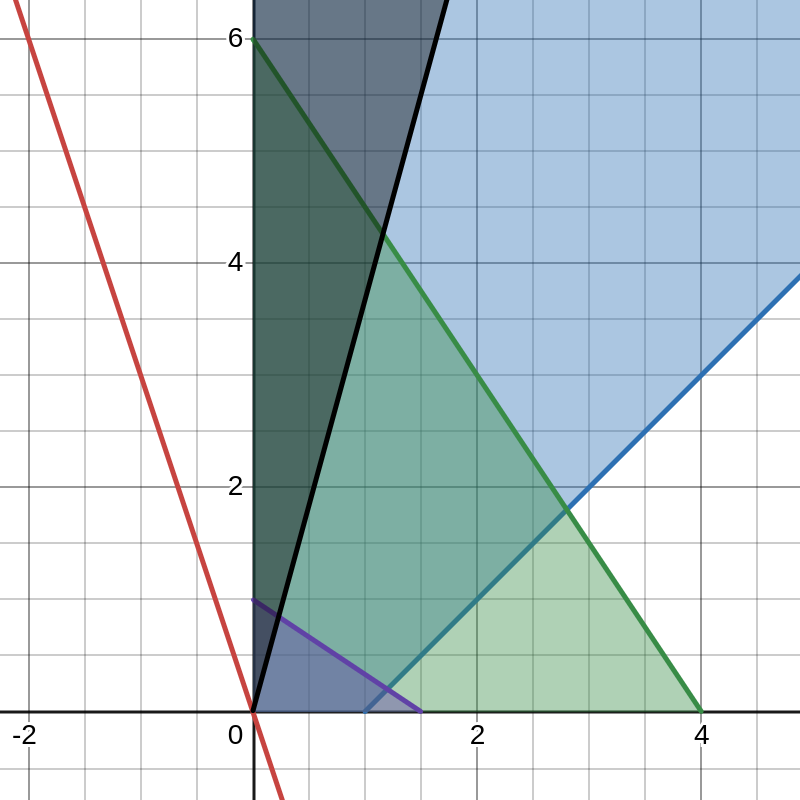
\includegraphics[scale = 0.35]{1.1(i).png}
    \end{figure}

Our red line is our objective function for $z = 0$ within the boundary of our feasible set, the dark triangle in our graph, our
minimum is $0$ with our minimizer being $(0,0)^T$. \newline
\textbf{\{ii\}}
    \begin{align*}
        \text{maximize} &\null \quad z = x_1 + 2x_2 \\ 
        \text{subject to} &\null \quad 2x_1 + x_2 \geq 12 \\
        & x_1 + x_2 \geq 5 \\
        & -x_1 + 3x_2 \leq 3 \\
        & 6x_1 - x_2 \geq 12 \\
        & x_1, x_2 \geq 0
    \end{align*}
    \begin{figure}[H]
        \centering
        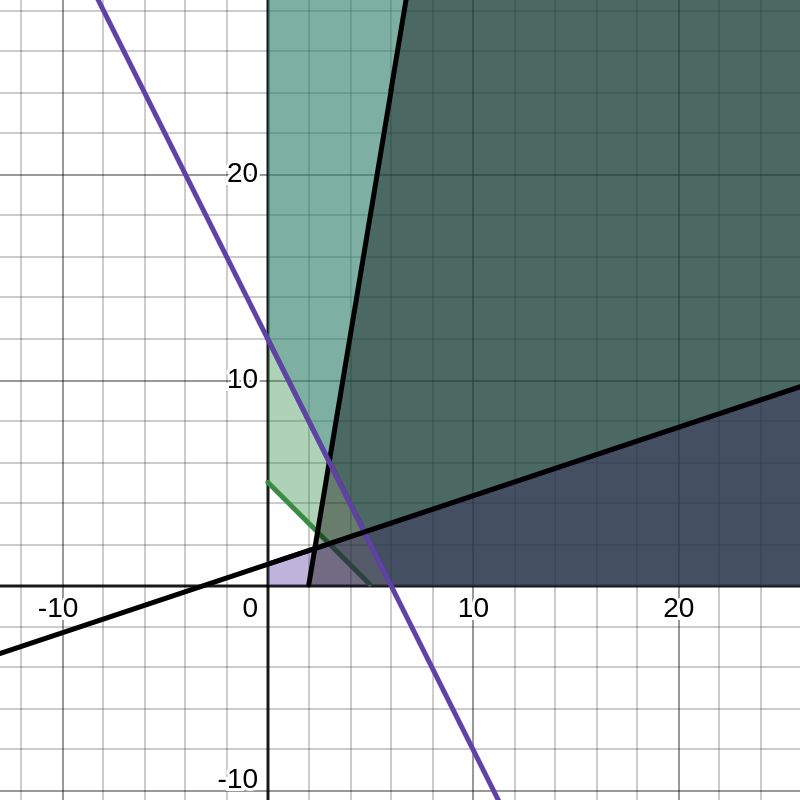
\includegraphics[scale = 0.35]{1.1(ii).png}
    \end{figure}

Our solution to this problem is bound by the constraint $-x_1 +3x_2 \leq 3$, Giving us our maximum value $z = 3$ along the line $-x_1 + 3x_2 = 3$. Our solution set ends up being  $p_2 = \frac{p_1}{3} + 1$ for $p_1 \geq \frac{33}{7}$ and $p_2 \geq \frac{18}{7}$.

\textbf{\{iii\}}
    \begin{align*}
        \text{minimize} &\null \quad z = x_1 - 2x_2 \\ 
        \text{subject to} &\null \quad x_1 - 2x_2 \geq 4 \\
        & x_1 + x_2 \leq 8 \\
        & x_1, x_2 \geq 0
    \end{align*}
    \begin{figure}[H]
        \centering
        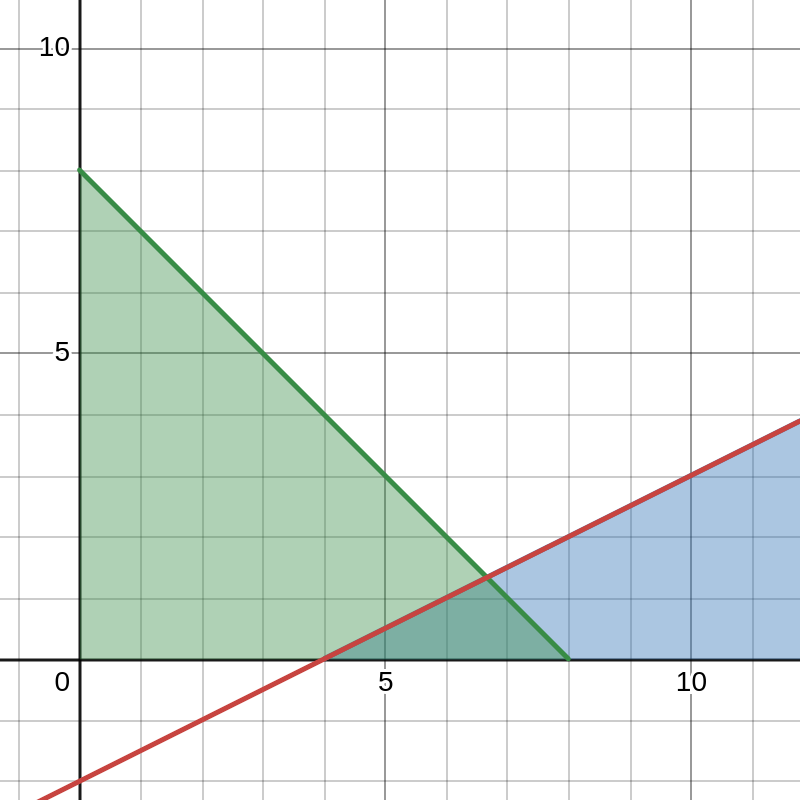
\includegraphics[scale = 0.35]{1.1(iii).png}
    \end{figure}

Our red line is our objective function for $z = 4$ and our feasible set is the darker green shaded triangle in our figure. our minimum value ends up being $4$ with our minimizer being the set of points along the red line on the triangle. the point $(4,0)^t$ is on the vertex is in our solution set for example. our solution set ends up being $p_2 = \frac{p_1}{2}-2$ for $p_1 \in [4, \frac{20}{3}]$ and $p_2 \in [0, \frac{4}{3}]$.

\textbf{\{iv\}}
    \begin{align*}
        \text{minimize} &\null \quad z = -x_1 - x_2 \\ 
        \text{subject to} &\null \quad x_1 - x_2 \geq 1 \\
        & x_1 - 2x_2 \leq 8 \\
        & x_1, x_2 \geq 0
    \end{align*}
    \begin{figure}[H]
        \centering
        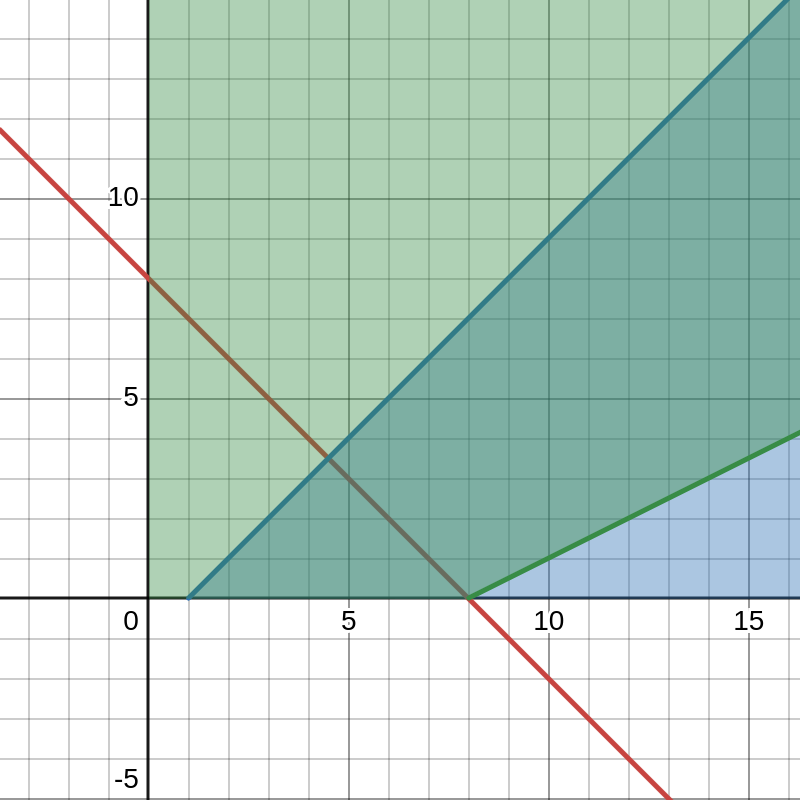
\includegraphics[scale = 0.35]{1.1(iv).png}
    \end{figure}

Our red line is our objective function for $z = -8$, our minimum ends up being $-8$ with our minimizer being $(8,0)^T$

\textbf{Problem 1.2} We are tasked with finding all values $a$ such that $(-3,4)^T$ us the optimal solution of the following problem:
\begin{align*}
  \text{maximize } && z = ax_1 + (2-a)x_2 \\
  \text{subject to } && 4x_1 + 3x_2 \leq 0 \\
  && 2x_1 + 3x_2 \leq 7 \\ 
  && x_1 + x_2 \leq 1
\end{align*}
We graph the function below
\begin{figure}[H]
    \centering
    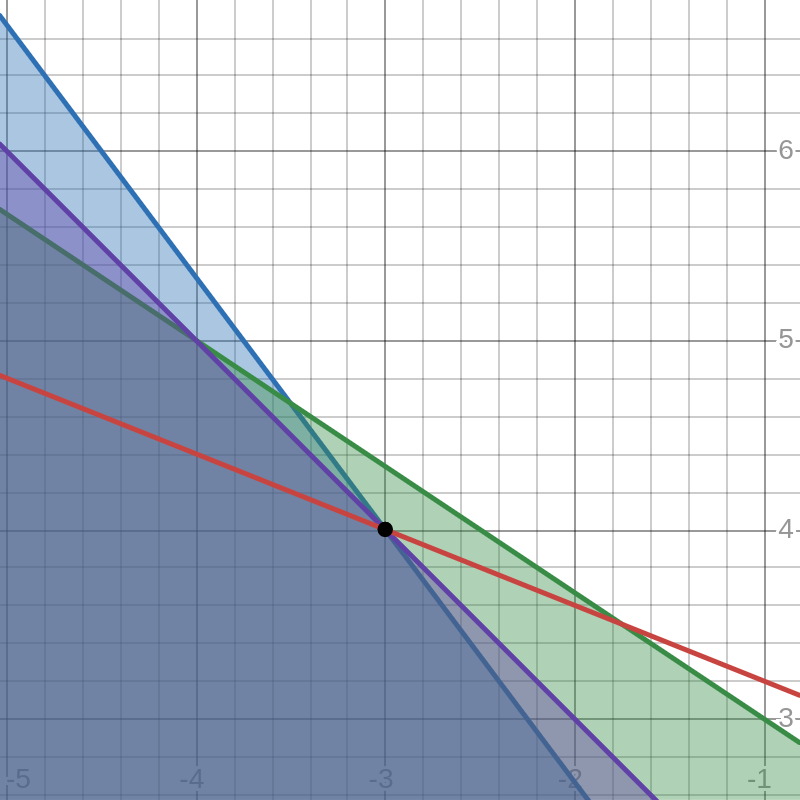
\includegraphics[scale = 0.35]{1.2.png}
\end{figure}
Our red line is objective function with $a = \frac{4}{7}$ and our, we found this a by plotting our point $(-3,4)^T$ and walking along $a$ values. We find that our $z$ grows larger and larger below that value of a. The range of a that maximizes our objective function for the given point we find is $a \in (-\infty, \frac{4}{7}] $. 

\end{document}
